\section{Grouped lasso}
\textit{Afsnittet er skrevet udfra kapitel 4 i \citep{hastie}}. \\[4mm]
%
I mange regressions problemer har prædiktorerne en naturlig grupperet struktur, og da foretrækkes det at alle koefficienter indenfor en gruppe er ikke-nul (eller nul) samtidig.

Betragt en lineær regressions model med $J$ grupper, hvor vektoren $Z_j \in \R^{p_j}$ for $j=1, \ldots, J$ repræsenterer prædiktorerne i gruppe $j$.
Formålet er da, at prædiktere responsvariablen $Y \in \R$ baseret på en samling af prædiktorer $(Z_1,\ldots,Z_J)$.
%En lineær model for regressions funktionen $\E{Y \vert Z}$ er givet ved \(\theta_0 + \sum_{j=1}^J Z_j^T \theta_j\), hvor $\theta_j \in \R^{p_j}$ repræsenterer en gruppe af $p_j$ regressions koefficienter. 

Given en samling af $n$ samples \(\{(y_i, z_{i,1}, z_{i,2}, \ldots, z_{i,J})\}_{i=1}^n\) løser group lasso følgende optimeringsproblem
\begin{align}
\beta^{\text{group lasso}} = \argmin_{\theta_j \in \R^{p_j}} \cbr{\frac{1}{2} \sum_{i=1}^n \del{y_i - \sum_{j=1}^J z_{ij}^T \theta_j}^2 + \lambda \sum_{j=1}^J \Vert \theta_j \Vert_2}. \label{eq:4.5}
\end{align}
Dette er en grupperet generalisering af lasso, som har følgende egenskaber:
\begin{itemize}
\item Afhængig af $\lambda$, vil enten alle indgange i vektoren $\hat{\theta}_j$ være nul eller ikke-nul
\item Når $p_j=1$, da har vi at $\Vert \theta_j \Vert_2 = \vert \theta_j \vert$, således at alle grupper er singletons, dermed reduceres optimeringsproblemet \eqref{eq:4.5} til standard lasso.
\end{itemize}
Figur \ref{fig:elastisk_net} viser betingelsesområderne for henholdsvis group lasso og standard lasso for tre variable.
%Vi ser at den grupperet lasso deler egenskaber med både $\ell_1$ og $\ell_2$ kuglen.
%
\begin{figure}[H]
\centering
 \scalebox{0.5}{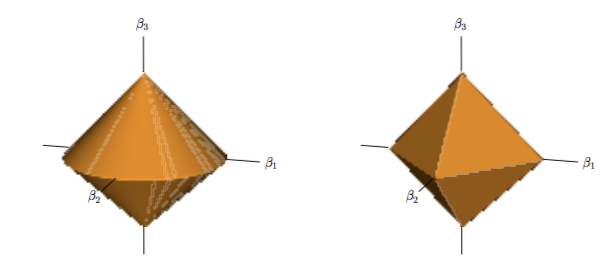
\includegraphics{fig/group_lasso.jpg}}
\caption{Til venstre ses kuglen for elastisk net med \(\alpha=0.7\) og til højre ses \(\ell_1\) kuglen for \(p=3\).}
\label{fig:elastisk_net}
\end{figure}
%
I \eqref{eq:4.5}, straffes alle grupper ligeligt, hvilket betyder at større grupper vil have en tendens til at blive valgt.
\citep{group_lasso} anbefalede at vægte strafleddene for hver gruppe i forhold til gruppens størrelse med en factor \(\sqrt{p_j}\).

\subsection{Udregning af group lasso}
\subsubsection{Coordinate descent}
Lad os omskrive optimeringsproblemet \eqref{eq:4.5} på matrix-vektor form
\begin{align*}
\argmin_{\theta_1, \ldots, \theta_J} \cbr{\frac{1}{2} \Vert \y - \sum_{j=1}^J \mathbf{Z}_{j} \theta_j \Vert_2^2 + \lambda \sum_{j=1}^J \Vert \theta_j \Vert_2}.
\end{align*}
For dette problem er nul subgradient ligningerne givet ved
\begin{align*}
- \mathbf{Z}_{j}^T \del{\y - \sum_{\ell=1}^J \mathbf{Z}_\ell \hat{\theta}_\ell} + \lambda \hat{s}_j = 0, \quad j=1,\ldots, J,
\end{align*} 
hvor $\hat{s}_j \in \R^{p_j}$ er et element af subdifferentialet af normen $\Vert \cdot \Vert_2$ evalueret i $\hat{\theta}_j$.
Når $\hat{\theta}_j \neq 0$ da har vi, at $\hat{s}_j = \frac{\hat{\theta}_j}{\Vert \hat{\theta}_j \vert_2}$, og når $\hat{\theta}_j=0$ da har vi, at $\hat{s}_j$ er enhver vektor hvor $\Vert \hat{s}_j \Vert_2 \leq 1$.
En metode at løse nul subgradent ligningerne er ved at fastholde alle block vektorer $\{\hat{\theta}_k, k \neq j\}$, og da løse for $\hat{\theta}_j$.
Hermed udføres block coordinate descent på objektfunktionen af group lasso.
Da problemet er konveks, og strafleddet kan separeres efter block, er det garanteret at konvergere til en optimal løsning.

Med $\{\hat{\theta}_k, k \neq j\}$ fastholdt, kan vi skrive
\begin{align*}
- \mathbf{Z}_{j}^T \del{\mathbf{r}_j - \mathbf{Z}_j \hat{\theta}_j} + \lambda \hat{s}_j = 0,
\end{align*}
hvor $\mathbf{r}_j = \y - \sum_{k \neq j} \mathbf{Z}_k \hat{\theta}_k $ er den j'te partial residual.
Fra betingelserne opfyldt af subgradienten $\hat{s}_j$, må vi have at $\hat{\theta}_j =0$ hvis $\Vert \mathbf{Z}_j^T \mathbf{r}_j \Vert_2 < \lambda$, og ellers må $\hat{\theta}_j$ opfylde
\begin{align}
\hat{\theta}_j = \del{\mathbf{Z}_j^T \mathbf{Z}_j + \frac{\lambda}{\Vert \hat{\theta}_j \Vert_2} \mathbf{I}}^{-1} \mathbf{Z}_j^T \mathbf{r}_j. \label{eq:4.14}
\end{align}
Denne opdatering er ens med løsningen af ridge regression, bortset fra at den underliggende strafparameter afhænger af $\Vert \hat{\theta}_j \Vert_2$.
Ligning \eqref{eq:4.14} har desværre ikke en lukket løsning for $\hat{\theta}_j$, medmindre at $\mathbf{Z}_j$ er ortonormal. I dette special tilfælde har vi, at
\begin{align*}
\hat{\theta}_j = \del{1 - \frac{\lambda}{\Vert \mathbf{Z}_j^T \mathbf{r}_j \Vert_2}}_+  \mathbf{Z}_j^T \mathbf{r}_j.
\end{align*}
Algoritmen er stabil og vil normal nå en fornuftig konvergens tolerance indenfor få iterationer.
De computermæssig byrde vil stige voldsomt når antallet af prædiktorer stiger.


\subsubsection{LARS}

\subsection{Sparse group lasso}
kompromis mellem group lasso og lasso
\newpage